\index{Resultado|(}
\section{Resultado}
\subsection{Resultados de experimentaci\'on con diferentes n}
\begin{itemize}
\item
  \begin{itemize}
    \item Parametros de entrada:
	  \begin{itemize}
	    \item Span: 18
	    \item h: 1
	    \item n: 4
	    \item $c_i$: 0.5
	    \item Costo Unitario: 2000
	    \item FMax: 10
	  \end{itemize}
      \item Resultados:
	  \begin{itemize}
	    \item Costo Final: 2000
	    \item Pilares insertados: 0
	    \item Fuerza Maxima ejercida: F7 4
	  \end{itemize}
      \end{itemize} 
\item 
    \begin{itemize}
    \item Parametros de entrada:
	  \begin{itemize}
	    \item Span: 18
	    \item h: 1
	    \item n: 6
	    \item $c_i$: 0.5
	    \item Costo Unitario: 2000
	    \item FMax: 10
	  \end{itemize}
      \item Resultados:
	  \begin{itemize}
	    \item Costo Final: 2000
	    \item Pilares insertados: 0. No fue necesario.
	    \item Fuerza Maxima ejercida subpuente 1: F11 6.75
	  \end{itemize}
      \end{itemize}
\item
  \begin{itemize}
    \item Parametros de entrada:
	  \begin{itemize}
	    \item Span: 18
	    \item h: 1
	    \item n: 8
	    \item $c_1$: 0.5
	    \item $c_2$: 0.5
	    \item $c_3$: 0.5
	    \item $c_4$: 0.5
	    \item $c_5$: 0.5
	    \item Costo Unitario: 2000
	    \item FMax: 10
	  \end{itemize}
      \item Resultados:
	  \begin{itemize}
	    \item Costo Final: 2000
	    \item Pilares insertados: 0
	    \item Fuerza Maxima ejercida: F15 8
	  \end{itemize}
      \end{itemize}

\item
  \begin{itemize}
    \item Parametros de entrada:
	  \begin{itemize}
	    \item Span: 100
	    \item h: 1
	    \item n: 90
	    \item $c_i$: 0.5
	    \item Costo Unitario: 2000
	    \item FMax: 20
	  \end{itemize}
      \item Resultados:
	  \begin{itemize}
	    \item Costo Final: 48841.5
	    \item Pilares insertados: 7
	    \item Fuerza Maxima ejercida en uno de los subpuentes fue: F23 9
	    \item Obs: Para el resto de la FM\'ax, estuvieron acotadas por 9.
	  \end{itemize}
      \end{itemize}
\item
  \begin{itemize}
    \item Parametros de entrada:
	  \begin{itemize}
	    \item Span: 100
	    \item h: 1
	    \item n: 80
	    \item $c_i$: 0.5
	    \item Costo Unitario: 2000
	    \item FMax: 20
	  \end{itemize}
      \item Resultados:
	  \begin{itemize}
	    \item Costo Final: 41423.8
	    \item Pilares insertados: 7
	    \item Fuerza Maxima ejercida en uno de los subpuentes fue: F19 12.5
	    \item Obs: Para el resto de la FM\'ax, estuvieron acotadas por 12.5.
	  \end{itemize}
      \end{itemize}
\item
  \begin{itemize}
    \item Parametros de entrada:
	  \begin{itemize}
	    \item Span: 100
	    \item h: 1
	    \item n: 70
	    \item $c_i$: 0.5
	    \item Costo Unitario: 2000
	    \item FMax: 20
	  \end{itemize}
      \item Resultados:
	  \begin{itemize}
	    \item Costo Final: 34924.3
	    \item Pilares insertados: 7
	    \item Fuerza Maxima ejercida en uno de los subpuentes fue: F19 18.75
	    \item Obs: Para el resto de la FM\'ax, estuvieron acotadas por 12.
	  \end{itemize}
      \end{itemize}
\item
  \begin{itemize}
    \item Parametros de entrada:
	  \begin{itemize}
	    \item Span: 100
	    \item h: 1
	    \item n: 50
	    \item $c_i$: 0.5
	    \item Costo Unitario: 2000
	    \item FMax: 20
	  \end{itemize}
      \item Resultados:
	  \begin{itemize}
	    \item Costo Final: 25267.3
	    \item Pilares insertados: 4
	    \item Fuerza Maxima ejercida en uno de los subpuentes fue: F15 8
	    \item Obs: Para el resto de la FM\'ax, estuvieron acotadas por 4.5.
	  \end{itemize}
      \end{itemize}
\item
  \begin{itemize}
    \item Parametros de entrada:
	  \begin{itemize}
	    \item Span: 100
	    \item h: 1
	    \item n: 40
	    \item $c_i$: 0.5
	    \item Costo Unitario: 2000
	    \item FMax: 20
	  \end{itemize}
      \item Resultados:
	  \begin{itemize}
	    \item Costo Final: 21307.2
	    \item Pilares insertados: 3
	    \item Fuerza Maxima ejercida en uno de los subpuentes fue: F19 18.75
	    \item Obs: Para el resto de la FM\'ax, estuvieron acotadas por 18.75.
	  \end{itemize}
      \end{itemize}
\item
  \begin{itemize}
    \item Parametros de entrada:
	  \begin{itemize}
	    \item Span: 100
	    \item h: 1
	    \item n: 10
	    \item $c_i$: 0.5
	    \item Costo Unitario: 2000
	    \item FMax: 20
	  \end{itemize}
      \item Resultados:
	  \begin{itemize}
	    \item Costo Final: 5818.29
	    \item Pilares insertados: 2
	    \item Fuerza Maxima ejercida el subpuente de la seccion 1: F7 10
	    \item Fuerza Maxima ejercida el subpuente de la seccion 2: F6 -5.07544
	    \item Fuerza Maxima ejercida el subpuente de la seccion 3: F7 10
	  \end{itemize}
      \end{itemize}	
\item
  \begin{itemize}
    \item Parametros de entrada:
	  \begin{itemize}
	    \item Span: 100
	    \item h: 1
	    \item n: 6
	    \item $c_i$: 0.5
	    \item Costo Unitario: 2000
	    \item FMax: 20
	  \end{itemize}
      \item Resultados:
	  \begin{itemize}
	    \item Costo Final: 2000
	    \item Pilares insertados: 1
	    \item Fuerza Maxima ejercida el subpuente de la seccion 1: F6 -9.04174
	    \item Fuerza Maxima ejercida el subpuente de la seccion 2: F7 17
	  \end{itemize}
      \end{itemize}
\end{itemize}
\subsection{Resultados de experimentaci\'on con diferentes Fuerzas M\'aximas}
\begin{itemize}
\item
  \begin{itemize}
    \item Parametros de entrada:
	  \begin{itemize}
	    \item Span: 18
	    \item h: 1
	    \item n: 6
	    \item $c_i$: 0.5
	    \item Costo Unitario: 2000
	    \item FMax: 5
	  \end{itemize}
      \item Resultados:
	  \begin{itemize}
	    \item Costo Final: 2000
	    \item Pilares insertados: 1
	    \item Fuerza Maxima ejercida en el subpuente 1 de 2 secciones: F6 -1.76744
	    \item Fuerza Maxima ejercida en el subpuente 2 de 4 secciones: F7 3
	  \end{itemize}
      \end{itemize}
\item
  \begin{itemize}
    \item Parametros de entrada:
	  \begin{itemize}
	    \item Span: 18
	    \item h: 1
	    \item n: 6
	    \item $c_i$: 0.5
	    \item Costo Unitario: 2000
	    \item FMax: 10
	  \end{itemize}
      \item Resultados:
	  \begin{itemize}
	    \item Costo Final: 2000
	    \item Pilares insertados: 0
	    \item Fuerza Maxima ejercida: F11 6.75
	  \end{itemize}
      \end{itemize}
\item
  \begin{itemize}
    \item Parametros de entrada:
	  \begin{itemize}
	    \item Span: 18
	    \item h: 1
	    \item n: 6
	    \item $c_i$: 0.5
	    \item Costo Unitario: 2000
	    \item FMax: 3
	  \end{itemize}
      \item Resultados:
	  \begin{itemize}
	    \item Costo Final: 2000
	    \item Pilares insertados: 1
	    \item Fuerza Maxima ejercida en el subpuente 1 de 2 secciones: F6 -1.76744
	    \item Fuerza Maxima ejercida en el subpuente 2 de 4 secciones: F7 3
	  \end{itemize}
      \end{itemize}
\item
  \begin{itemize}
    \item Parametros de entrada:
	  \begin{itemize}
	    \item Span: 18
	    \item h: 1
	    \item n: 6
	    \item $c_i$: 0.5
	    \item Costo Unitario: 2000
	    \item FMax: 2
	  \end{itemize}
      \item Resultados:
	  \begin{itemize}
	    \item Costo Final: 4235.54
	    \item Pilares insertados: 2
	    \item Fuerza Maxima ejercida en el subpuente 1 de 2 secciones: F6 -1.76744
	    \item Fuerza Maxima ejercida en el subpuente 2 de 2 secciones: F6 -1.76744
	    \item Fuerza Maxima ejercida en el subpuente 2 de 2 secciones: F6 -1.76744
	  \end{itemize}
      \end{itemize}
\item
  \begin{itemize}
    \item Parametros de entrada:
	  \begin{itemize}
	    \item Span: 18
	    \item h: 1
	    \item n: 6
	    \item $c_i$: 0.5
	    \item Costo Unitario: 2000
	    \item FMax: 1
	  \end{itemize}
      \item Resultados:
	  \begin{itemize}
	    \item Costo Final: 4235.54
	    \item Pilares insertados: 2
	    \item Fuerza Maxima ejercida en el subpuente 1 de 2 secciones: F6 -1.76744
	    \item Fuerza Maxima ejercida en el subpuente 2 de 2 secciones: F6 -1.76744
	    \item Fuerza Maxima ejercida en el subpuente 2 de 2 secciones: F6 -1.76744
	    \item Obs: En este caso result\'o extraño. Con fuerzas m\'aximas muy pequeñas no se puede construir el puente. habr\'ia que insertar un pilar
por cada secci\'on del mismo.
	  \end{itemize}
      \end{itemize}
\subsection{Resultados de experimentaci\'on con Span muy grande:}
\item
  \begin{itemize}
    \item Parametros de entrada:
	  \begin{itemize}
	    \item Span: 100
	    \item h: 1
	    \item n: 6
	    \item $c_i$: 0.5
	    \item Costo Unitario: 2000
	    \item FMax: 20
	  \end{itemize}
      \item Resultados:
	  \begin{itemize}
	    \item Costo Final: 2000
	    \item Pilares insertados: 1
	    \item Fuerza Maxima ejercida en el subpuente 1 de 2 secciones: F6 -9.04174
	    \item Fuerza Maxima ejercida en el subpuente 2 de 4 secciones: F7 17
	  \end{itemize}
      \end{itemize}
\item
  \begin{itemize}
    \item Parametros de entrada:
	  \begin{itemize}
	    \item Span: 100
	    \item h: 1
	    \item n: 100
	    \item $c_i$: 0.5
	    \item Costo Unitario: 2000
	    \item FMax: 20
	  \end{itemize}
      \item Resultados:
	  \begin{itemize}
	    \item Costo Final: 57106.7
	    \item Pilares insertados: 7
	    \item Fuerza Maxima ejercida en uno de los subpuentes fue: F27 12.25
	    \item Obs: Para el resto de la FM\'ax, estuvieron acotadas por 9.
	  \end{itemize}
      \end{itemize}
\item
  \begin{itemize}
    \item Parametros de entrada:
	  \begin{itemize}
	    \item Span: 100
	    \item h: 100
	    \item n: 100
	    \item $c_i$: 0.5
	    \item Costo Unitario: 2000
	    \item FMax: 20
	  \end{itemize}
      \item Resultados:
	  \begin{itemize}
	    \item Costo Final: 119083
	    \item Pilares insertados: 30
	    \item Fuerza Maxima ejercida en uno de los subpuentes fue: F3 19.0135
	    \item Obs: Para el resto de la FM\'ax, estuvieron acotadas por F2 -0.510308.
	  \end{itemize}
      \end{itemize}
\item
  \begin{itemize}
    \item Parametros de entrada:
	  \begin{itemize}
	    \item Span: 100
	    \item h: 50
	    \item n: 100
	    \item $c_i$: 0.5
	    \item Costo Unitario: 2000
	    \item FMax: 20
	  \end{itemize}
      \item Resultados:
	  \begin{itemize}
	    \item Costo Final: 89834.9
	    \item Pilares insertados: 30
	    \item Fuerza Maxima ejercida en uno de los subpuentes fue: F3 19.0163
	    \item Obs: Para el resto de la FM\'ax, estuvieron acotadas por F2 -0.510308.
	  \end{itemize}
      \end{itemize}
\item
  \begin{itemize}
    \item Parametros de entrada:
	  \begin{itemize}
	    \item Span: 100
	    \item h: 25
	    \item n: 100
	    \item $c_i$: 0.5
	    \item Costo Unitario: 2000
	    \item FMax: 20
	  \end{itemize}
      \item Resultados:
	  \begin{itemize}
	    \item Costo Final: 2000
	    \item Pilares insertados: 1
	    \item Fuerza Maxima ejercida en el subpuente 1 de 50 secciones: F198 12.2598
	    \item Fuerza Maxima ejercida en el subpuente 2 de 50 secciones: F198 12.2598
	  \end{itemize}
      \end{itemize}
\item
  \begin{itemize}
    \item Parametros de entrada:
	  \begin{itemize}
	    \item Span: 100
	    \item h: 5
	    \item n: 100
	    \item $c_i$: 0.5
	    \item Costo Unitario: 2000
	    \item FMax: 20
	  \end{itemize}
      \item Resultados:
	  \begin{itemize}
	    \item Costo Final: 124394
	    \item Pilares insertados: 3
	    \item Fuerza Maxima ejercida en uno de los subpuentes fue: F51 8.45
	    \item Obs: Para el resto de la FM\'ax, estuvieron acotadas por F47 7.2.
	  \end{itemize}
      \end{itemize}
\item
  \begin{itemize}
    \item Parametros de entrada:
	  \begin{itemize}
	    \item Span: 100
	    \item h: 8
	    \item n: 100
	    \item $c_i$: 0.5
	    \item Costo Unitario: 2000
	    \item FMax: 20
	  \end{itemize}
      \item Resultados:
	  \begin{itemize}
	    \item Costo Final: 2000
	    \item Pilares insertados: 1
	    \item Fuerza Maxima ejercida en el subpuente 1 de 50 secciones: F99 19.5312
	    \item Fuerza Maxima ejercida en el subpuente 2 de 50 secciones: F99 19.5312
	  \end{itemize}
      \end{itemize}
\item
  \begin{itemize}
    \item Parametros de entrada:
	  \begin{itemize}
	    \item Span: 100
	    \item h: 30
	    \item n: 100
	    \item $c_i$: 0.5
	    \item Costo Unitario: 2000
	    \item FMax: 20
	  \end{itemize}
      \item Resultados:
	  \begin{itemize}
	    \item Costo Final: 38136.9
	    \item Pilares insertados: 10
	    \item Fuerza Maxima ejercida en uno de los subpuentes fue: F3 19.761
	    \item Obs: Para el resto de la FM\'ax, estuvieron acotadas por F2 -0.517539.
	  \end{itemize}
      \end{itemize}
\item
  \begin{itemize}
    \item Parametros de entrada:
	  \begin{itemize}
	    \item Span: 100
	    \item h: 1
	    \item n: 100
	    \item $c_i$: 0.5
	    \item Costo Unitario: 2000
	    \item FMax: 50
	  \end{itemize}
      \item Resultados:
	  \begin{itemize}
	    \item Costo Final: 49106.7
	    \item Pilares insertados: 3
	    \item Fuerza Maxima ejercida en uno de los subpuentes fue: F51 42.25
	    \item Obs: Para el resto de la FM\'ax, estuvieron acotadas por F47 36.
	  \end{itemize}
      \end{itemize}
\item
  \begin{itemize}
    \item Parametros de entrada:
	  \begin{itemize}
	    \item Span: 100
	    \item h: 1
	    \item n: 100
	    \item $c_i$: 0.5
	    \item Costo Unitario: 2000
	    \item FMax: 200
	  \end{itemize}
      \item Resultados:
	  \begin{itemize}
	    \item Costo Final: 2000
	    \item Pilares insertados: 1
	    \item Fuerza Maxima ejercida en ambos subpuentes: F99 156.25
	  \end{itemize}
      \end{itemize}
\item
  \begin{itemize}
    \item Parametros de entrada:
	  \begin{itemize}
	    \item Span: 100
	    \item h: 1
	    \item n: 100
	    \item $c_i$: 0.5
	    \item Costo Unitario: 2000
	    \item FMax: 150
	  \end{itemize}
      \item Resultados:
	  \begin{itemize}
	    \item Costo Final: 49106.7
	    \item Pilares insertados: 3
	    \item Fuerza Maxima ejercida en uno de los subpuentes fue: F51 42.25
	    \item Obs: Para el resto de la FM\'ax, estuvieron acotadas por F47 36.
	  \end{itemize}
      \end{itemize}
\item
  \begin{itemize}
    \item Parametros de entrada:
	  \begin{itemize}
	    \item Span: 100
	    \item h: 1
	    \item n: 100
	    \item $c_i$: 0.5
	    \item Costo Unitario: 2000
	    \item FMax: 40
	  \end{itemize}
      \item Resultados:
	  \begin{itemize}
	    \item Costo Final: 53106.7
	    \item Pilares insertados: 5
	    \item Fuerza Maxima ejercida en uno de los subpuentes fue: F51 42.25
	    \item Obs: Para el resto de la FM\'ax, estuvieron acotadas por F47 36.
	  \end{itemize}
      \end{itemize}
\item
  \begin{itemize}
    \item Parametros de entrada:
	  \begin{itemize}
	    \item Span: 100
	    \item h: 1
	    \item n: 100
	    \item $c_i$: 0.5
	    \item Costo Unitario: 2000
	    \item FMax: 10
	  \end{itemize}
      \item Resultados:
	  \begin{itemize}
	    \item Costo Final: 61106.7
	    \item Pilares insertados: 9
	    \item Fuerza Maxima ejercida en uno de los subpuentes fue: F15 4
	    \item Obs: Para el resto de la FM\'ax, estuvieron acotadas por F11 2.25.
	  \end{itemize}
      \end{itemize}
\end{itemize}
\subsection{Resultados de experimentaci\'on con diferentes Fuerzas C}
\begin{itemize}
\item
  \begin{itemize}
    \item Parametros de entrada:
	  \begin{itemize}
	    \item Span: 100
	    \item h: 1
	    \item n: 100
	    \item $c_i$: 1
	    \item Costo Unitario: 2000
	    \item FMax: 20
	  \end{itemize}
      \item Resultados:
	  \begin{itemize}
	    \item Costo Final: 61106.7
	    \item Pilares insertados: 9
	    \item Fuerza Maxima ejercida en uno de los subpuentes fue: F15 8
	    \item Obs: Para el resto de la FM\'ax, estuvieron acotadas por F11 4.5.
	  \end{itemize}
      \end{itemize}
\item
  \begin{itemize}
    \item Parametros de entrada:
	  \begin{itemize}
	    \item Span: 100
	    \item h: 1
	    \item n: 100
	    \item $c_i$: 1.5
	    \item Costo Unitario: 2000
	    \item FMax: 20
	  \end{itemize}
      \item Resultados:
	  \begin{itemize}
	    \item Costo Final: 73106.7
	    \item Pilares insertados: 15
	    \item Fuerza Maxima ejercida en uno de los subpuentes fue: F15 12
	    \item Obs: Para el resto de la FM\'ax, estuvieron acotadas por F11 6.75.
	  \end{itemize}
      \end{itemize}
\item
  \begin{itemize}
    \item Parametros de entrada:
	  \begin{itemize}
	    \item Span: 100
	    \item h: 1
	    \item n: 100
	    \item $c_i$: 0.25
	    \item Costo Unitario: 2000
	    \item FMax: 20
	  \end{itemize}
      \item Resultados:
	  \begin{itemize}
	    \item Costo Final: 53106.7
	    \item Pilares insertados: 5
	    \item Fuerza Maxima ejercida en uno de los subpuentes fue: F27 6.125
	    \item Obs: Para el resto de la FM\'ax, estuvieron acotadas por F23 4.5.
	  \end{itemize}
      \end{itemize}
\end{itemize}

\subsection{Resultados de experimentaci\'on en funci\'on del span:}
\subsubsection{Parametros de entrada Fijos:}
los parametros que no var\'ian son:
  \begin{itemize}
      \item h: 1
      \item n: 6
      \item $c_i$: 0.2
      \item Costo Unitario: 2000
      \item FMax: 0.5
  \end{itemize}
\subsubsection{Resultados segun Span:}
  \begin{itemize}
   \item 
      \begin{itemize}
	\item span: 6
	\item Fuerza M\'axima resultante:0.8
      \end{itemize}
   \item 
      \begin{itemize}
	\item span: 10
	\item Fuerza M\'axima resultante:0.8
      \end{itemize}
   \item 
      \begin{itemize}
	\item span: 11
	\item Fuerza M\'axima resultante:0.8
      \end{itemize}
   \item 
      \begin{itemize}
	\item span: 12
	\item Fuerza M\'axima resultante:1.6
      \end{itemize}
   \item 
      \begin{itemize}
	\item span: 14
	\item Fuerza M\'axima resultante:1.6
      \end{itemize}
   \item 
      \begin{itemize}
	\item span: 16
	\item Fuerza M\'axima resultante:1.6
      \end{itemize}
   \item 
      \begin{itemize}
	\item span: 18
	\item Fuerza M\'axima resultante:2.4
      \end{itemize}
   \item 
      \begin{itemize}
	\item span: 24
	\item Fuerza M\'axima resultante:3.2
      \end{itemize}
  \end{itemize}
\begin{center}
 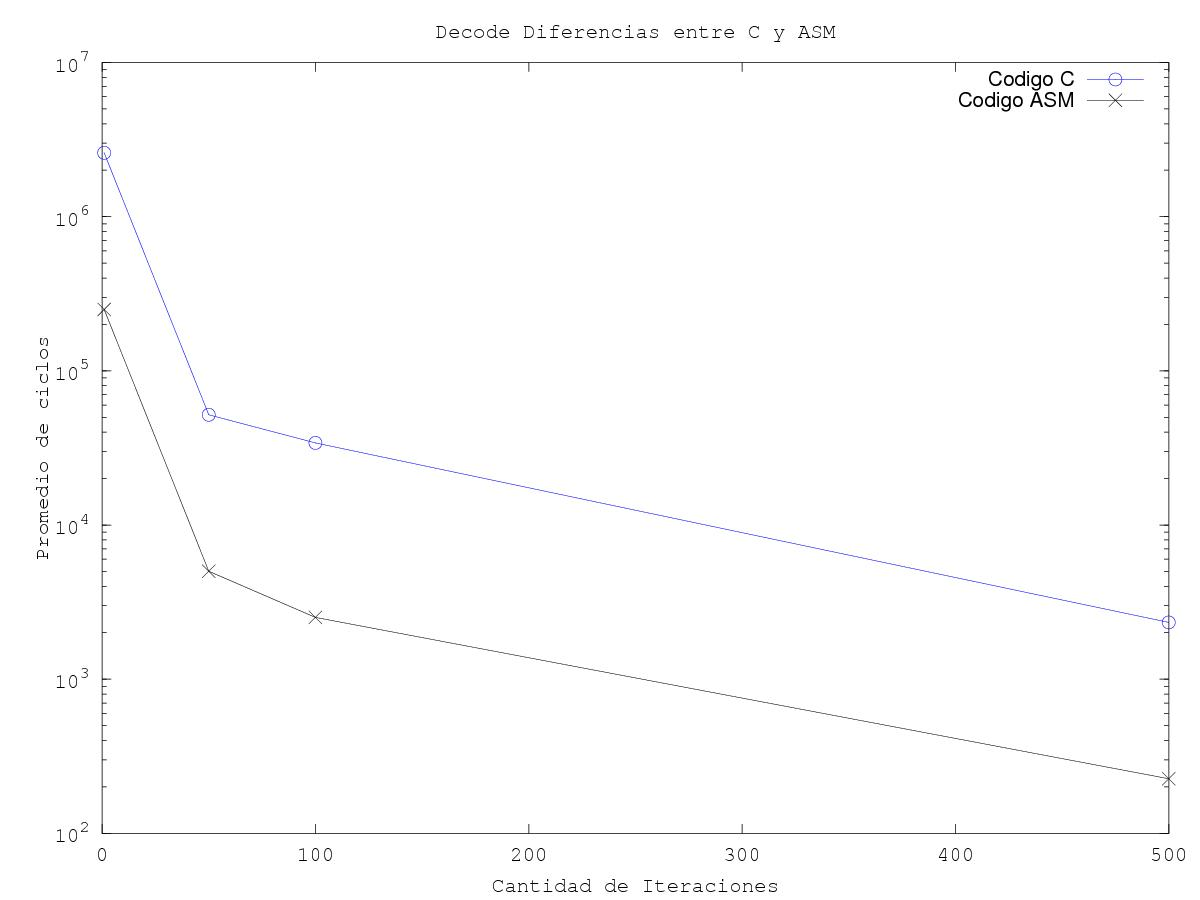
\includegraphics[scale=0.6]{imagenes/octave1.jpg}
\end{center}
\subsection{Resultados para experimentaci\'on variando n para distintas Fuerzas Máximas}
\subsubsection{Parametros de entrada Fijos:}
los parametros que no var\'ian son:
  \begin{itemize}
      \item span: 18
      \item h: 1
      \item $c_i$: 0.2
      \item Costo Unitario: 2000
      \item FMax: 0.5
  \end{itemize}
\subsubsection{Resultados segun n:}
  \begin{itemize}
   \item 
      \begin{itemize}
	\item n: 2
	\item Fuerza M\'axima resultante:F6 -1.83358
      \end{itemize}
   \item 
      \begin{itemize}
	\item n: 4
	\item Fuerza M\'axima resultante:F7 1.6
      \end{itemize}
   \item 
      \begin{itemize}
	\item n: 6
	\item Fuerza M\'axima resultante:F11 2.7
      \end{itemize}
   \item 
      \begin{itemize}
	\item n: 8
	\item Fuerza M\'axima resultante:F15 3.2
      \end{itemize}
   \item 
      \begin{itemize}
	\item n: 10
	\item Fuerza M\'axima resultante:F19 2.5
      \end{itemize}
   \item 
      \begin{itemize}
	\item n: 12
	\item Fuerza M\'axima resultante:F23 3.6
      \end{itemize}
   \item 
      \begin{itemize}
	\item n: 14
	\item Fuerza M\'axima resultante:F27 4.9
      \end{itemize}
   \item 
      \begin{itemize}
	\item n: 16
	\item Fuerza M\'axima resultante:F31 6.4
      \end{itemize}
   \item 
      \begin{itemize}
	\item n: 18
	\item Fuerza M\'axima resultante:F35 8.1
      \end{itemize}
  \end{itemize}
  \begin{center}
 \includegraphics[scale=0.6]{imagenes/octave2.jpg}
\end{center}
\subsection{Resultados para experimentaci\'on variando C para distintas Fuerzas Máximas}
\subsubsection{Parametros de entrada Fijos:}
los parametros que no var\'ian son:
  \begin{itemize}
      \item span: 18
      \item h: 1
      \item n: 6
      \item Costo Unitario: 2000
      \item FMax: 0.5
  \end{itemize}
\subsubsection{Resultados segun n:}
\begin{itemize}
    \item 
      \begin{itemize}
	\item $C_i$: 0.1
	\item Fuerza M\'axima resultante:F11 1.35
      \end{itemize}
    \item 
      \begin{itemize}
	\item $C_i$: 0.5
	\item Fuerza M\'axima resultante:F11 6.75
      \end{itemize}
    \item 
      \begin{itemize}
	\item $C_i$: 1
	\item Fuerza M\'axima resultante: F11 13.5
      \end{itemize}
    \item 
      \begin{itemize}
	\item $C_i$: 1.5
	\item Fuerza M\'axima resultante:F11 20.25
      \end{itemize}
    \item 
      \begin{itemize}
	\item $C_i$: 15
	\item Fuerza M\'axima resultante:F11 202.5
      \end{itemize}
\end{itemize}
  \begin{center}
 \includegraphics[scale=0.6]{imagenes/octave3.jpg}
\end{center}
\index{Resultado|)}